%===============================================================================
% Template Name:      Advanse Group Template
% Template URI:       
% Description:        DC-UFSCar
%                  
% Version:            1.0
% Author:             Daniel San Martín
% License:            MIT License
% License URI:        http://opensource.org/licenses/MIT
%===============================================================================
\documentclass[serif,11pt,usenames,dvipsnames]{beamer}{\tiny }
\usetheme{advanse}
%========================
% load packages
%========================
\usepackage{tabularx}

%========================
% funding institution's logo
%========================
\titlegraphic{
	\begin{tikzpicture}[remember picture, overlay]
		\node[anchor=west] at (-5.8,0.5){\pgfuseimage{fund}};
	\end{tikzpicture}	
}

\title[Short title]{ Long Title of Your Presentation}
\author[Your Name --- {\sc Month day\superscript{th}, Year}]{Your Name}
\institute{PhD Advisor: Valter Vieira de Camargo \\ Advanse Group \\ Department of Computing, UFSCar \\ São Carlos, SP, Brazil}
\date{\today}

\begin{document}

%========================
% title page
%========================
\begin{frame}
	\titlepage
\end{frame}
%========================
%Table of Contents
%========================
\begin{frame}\frametitle{Outline}
\tableofcontents
\end{frame}
%========================
%Slides
%========================
\section{Introduction}
\subsection{Context}
\begin{frame}\frametitle{Adaptive Systems (ASs)}

\begin{figure}
	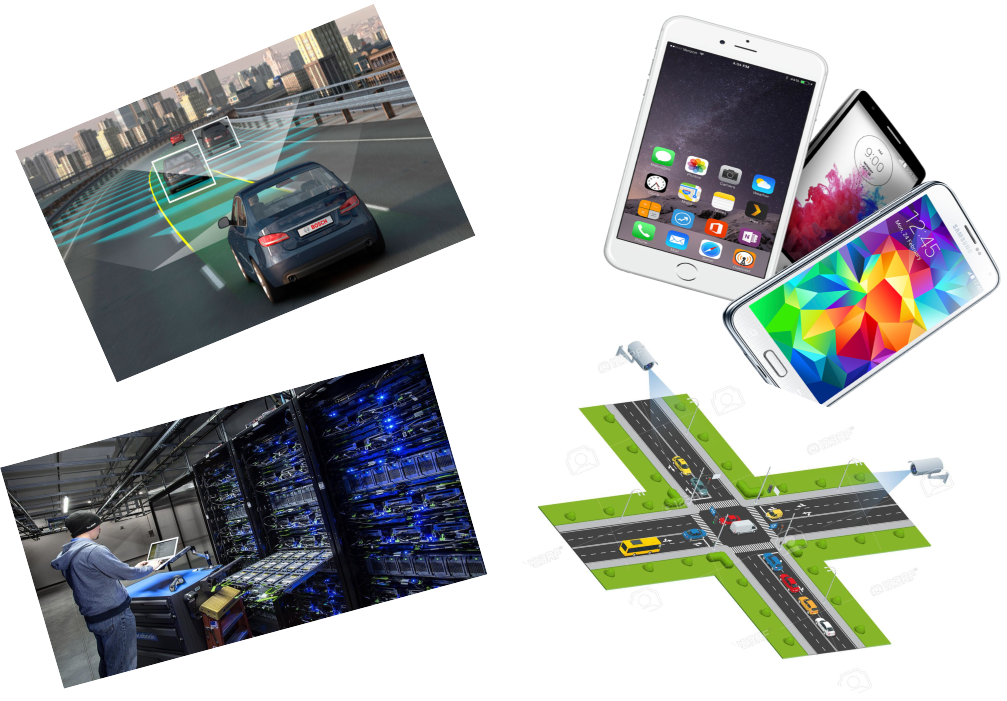
\includegraphics[width=0.8\textwidth]{figures/sas.png}
	\caption{Adaptive Systems are demanded in several domains}
\end{figure}

\end{frame}

\begin{frame}\frametitle{The implementation of ASs}
\begin{figure}
	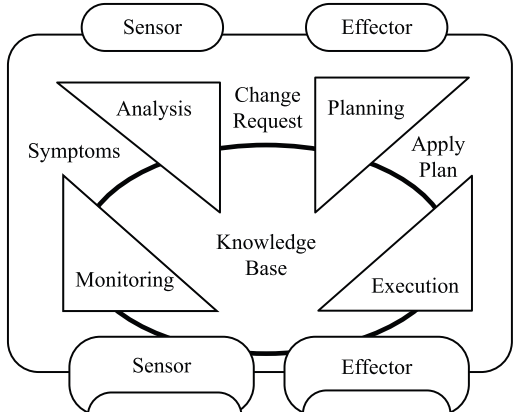
\includegraphics[width=0.7\textwidth]{figures/mapek.png}
	\caption{The autonomic reference model \cite{ibm2005architectural}}
\end{figure}

\end{frame}

\begin{frame}\frametitle{The implementation of ASs}

\textit{``Something in architecture design and its implementation is no longer adequate.''} \cite{Zimmermann2017}

\begin{figure}
	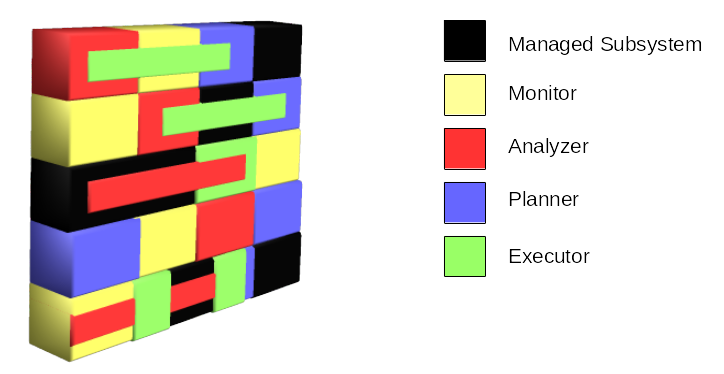
\includegraphics[width=0.8\textwidth]{figures/concern.png}
	\caption{AS abstractions are not evident in source code}
\end{figure}

\end{frame}

\begin{frame}\frametitle{Motivations}

\begin{itemize}
	\item Software engineers do not follow architectural models of ASs;
	\vspace{0.5cm}
	\item The lack of architectural smells catalogs of ASs;
	\vspace{0.5cm}
	\item The lack of approaches for identifying architectural smells of ASs.
\end{itemize}

\end{frame}
\subsection{Objectives}
\begin{frame}\frametitle{Objectives}

\begin{block}{Objective I}
	Characterizing architectural smells in the context of ASs.

\end{block}
\vspace{0.5cm}
\pause
\begin{block}{Objective II}
	Identifying a set of architectural smells of ASs. 
\end{block}
\vspace{0.5cm}
\pause

\begin{block}{Objective III}
	Supporting software engineers on the identification of architectural smells of ASs.
\end{block}


\end{frame}

\subsection{Contributions}
\begin{frame}\frametitle{Contributions}


\tikzstyle{q} = [rectangle, draw, fill=RoyalBlue, node distance=2cm, text width=12em,  text=white, rounded corners, minimum height=3em, thick]

\tikzstyle{r} = [rectangle, draw, fill=green!50!black, node distance=2cm, text width=12em,  text=white, rounded corners, minimum height=3em, minimum width=6em, thick]

\tikzstyle{v} = [rectangle, draw, fill=white, node distance=2cm, text width=10em, text centered,  rounded corners, minimum height=3em, minimum width=10em, thick]

\tikzstyle{l} = [draw, -latex',thick]

\begin{tikzpicture}
\node[q] (g1) at (0,0) {\textbf{Objective 1:}\\	{\scriptsize \textbf{Characterizing architectural smells in the context of ASs}}};
\node [q, below = 0.5cm of g1] (g2) {\textbf{Objective 2:}\\	{\scriptsize \textbf{Identifying a set of architectural smells of ASs}}};
\node [q, below = 0.5cm of g2] (g3) {\textbf{Objective 3:}\\	{\scriptsize \textbf{Supporting software engineers on the identification of architectural smells of ASs}}};


\node [r, right= 0.5cm of g1] (c1) {\textbf{Contribution 1:} \\ {\scriptsize \textbf{A catalog with formal and informal specifications}}};
\node [r, right= 0.5cm of g2] (c2) {\textbf{Contribution 2:} \\ {\scriptsize \textbf{A set of rules for applying on the identification of the smells}}};
\node [r, right= 0.5cm of g3] (c3) {\textbf{Contribution 3:} \\ {\scriptsize \textbf{A semi-automated tool for applying the identification rules}}};


\path [l] (g1) -- (c1);
\path [l] (g2) --  (c2);
\path [l] (g3) --  (c3);


\end{tikzpicture}


\end{frame}


\section{Background}
\begin{frame}\frametitle{Background Overview}

\centering
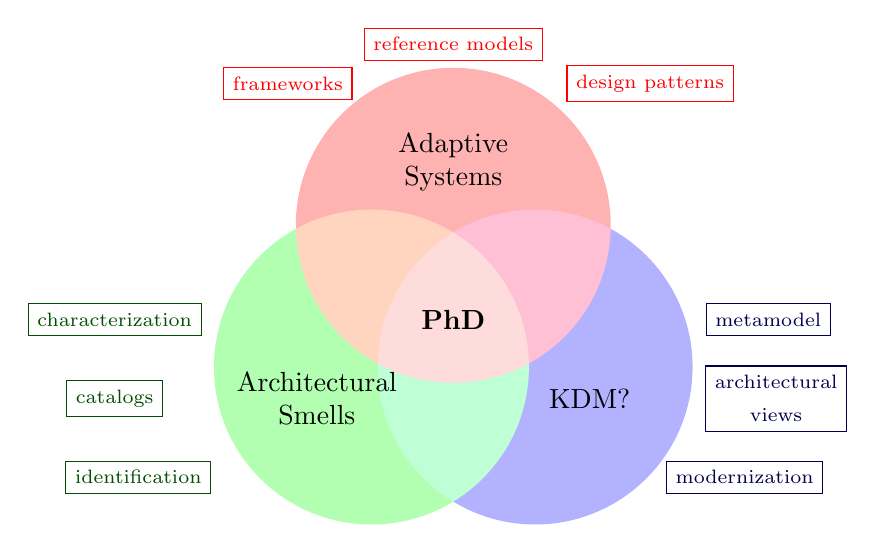
\begin{tikzpicture}
\onslide<1-> {

\begin{scope}[blend group = soft light]
\fill[red!30!white]   ( 90:1.2) circle (2);
\fill[green!30!white] (210:1.2) circle (2);
\fill[blue!30!white]  (330:1.2) circle (2);
\end{scope}


\node[align = center] at ( 90:2)    {Adaptive \\ Systems};
\node[align = center] at ( 210:2)   {Architectural \\ Smells};
\node[align = center] at ( 330:2)   {KDM?};
\node  {\textbf{PhD}};

}

\onslide<2-> {

\node[align = center, draw, rectangle, color= red] at ( -2.1,3)    {{\scriptsize frameworks}};
\node[align = center, draw, rectangle, color= red] at ( 0,3.5)    {{\scriptsize reference models}};
\node[align = center, draw, rectangle, color= red] at ( 2.5,3)    {{\scriptsize design patterns}};
}

\onslide<3-> {

\node[align = center, draw, rectangle, color= green!30!black] at (-4.3,0) {{\scriptsize characterization}}; 

\node[align = center, draw, rectangle, color= green!30!black] at (-4.3,-1) {{\scriptsize catalogs}};

\node[align = center, draw, rectangle, color= green!30!black] at (-4.0,-2) {{\scriptsize identification}};
}

\onslide<4->{

\node[align = center, draw, rectangle, color= blue!30!black] at (4.0,0) {{\scriptsize metamodel}};

\node[align = center, draw, rectangle, color= blue!30!black] at (4.1,-1) {{\scriptsize architectural} \\ {\scriptsize views}};

\node[align = center, draw, rectangle, color= blue!30!black] at (3.7,-2) {{\scriptsize modernization}};

}

\end{tikzpicture} 

\end{frame}

\section{Methodology}
\begin{frame}\frametitle{The Process}

\begin{tikzpicture}

\tikzstyle{p} = [rectangle, draw, node distance=2cm, text width=15em,  text=white, rounded corners, minimum height=3em, thick, color= red]

\tikzstyle{q} = [rectangle, draw, node distance=2cm, text width=15em,  text=white, rounded corners, minimum height=3em, thick, color= blue]
\tikzstyle{r} = [rectangle, draw, node distance=2cm, text width=15em,  text=white, rounded corners, minimum height=3em, thick, color= green]

\node[anchor=south west,inner sep=0] at (0,0)  {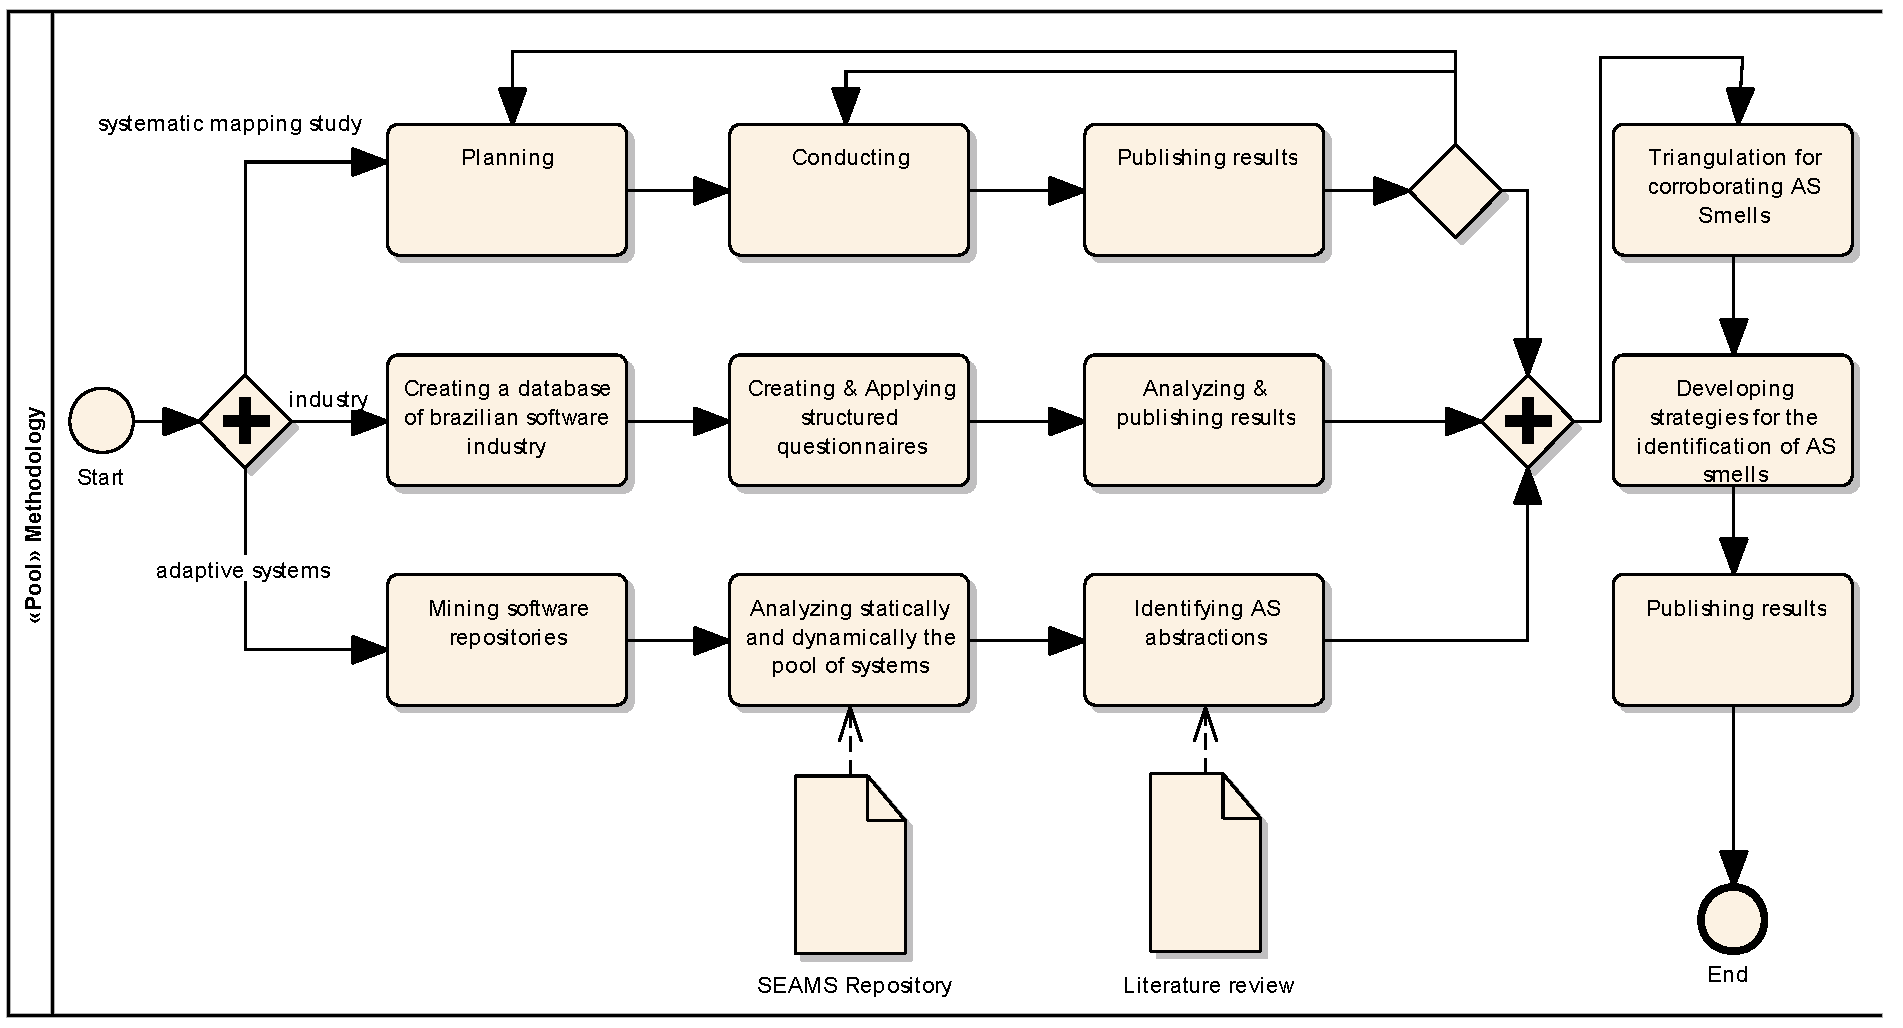
\includegraphics[width=\textwidth]{figures/process.pdf}};

\onslide<1-> {
\node[p] (a) at (4.8,4.8) {};
}

\onslide<2-> {

\node[q] (b) at (4.8,3.5) {};
}

\onslide<3-> {
\node[r] (c) at (4.8,2.2) {};
}
\end{tikzpicture}



\end{frame}


\begin{frame}\frametitle{Evaluation}


\begin{itemize}
	\justifying
	\item Controlled experiments in order to measure the required effort when software engineers need to perform maintenance tasks when there are presence of architectural smells of ASs.
	\vspace{0.5cm}
	\item Precision and recall metrics in order to measure the effectiveness of our set of identification rules for architectural smells of ASs.
	
\end{itemize}

\end{frame}

\section{Results}
\begin{frame}\frametitle{Systematic Mapping Study}
\newcolumntype{s}{>{\hsize=.1\hsize}X}

	\begin{table}[t]\tiny
		\centering
		\begin{tabularx}{\linewidth}{X|s|X}
			\hline
			\textbf{Architectural Smell}  &  \textbf{Cit.} & \textbf{Domain} \\ \hline
			Implicit Comunal Components   & 1 &Automotive - Embedded System\\
			Undesired extension of control software functionality   &1& Automated Production System (aPS) \\
			Extraneous Connector   &2& Automotive - Embedded System/Mobile\\
			Misplaced Logical Component (LC)   &1&Automotive - Embedded System\\
			Inconsistent hierarchical (de)composition &1&Mobile (Android)\\
			Extensibility limitations   &1&Mobile (Android)\\
			Omission of architectural concepts   &1&Mobile (Android)\\
			Model-view-controller anti-pattern   &1&Mobile (Android)\\
			Obscure Monitor   &1&Mobile (Android)\\
			Oppressed Monitor   &1&Mobile (Android)\\
			\hline
		\end{tabularx}
		\caption{Architectural smells found in literature related to adaptive systems}
	\end{table}
\end{frame}


%========================
% bibliography
%========================
\section{References}
\begin{frame}[allowframebreaks] \frametitle{References}
    \bibliographystyle{ieeetr}
    \bibliography{bibliography/bibliography}\vspace{0.1in}
\end{frame}

%=================================================
% end presentation
%=================================================
\section*{}
\begin{frame}{}
\centering \Huge
\emph{Thank You, Questions?}
\end{frame}

\end{document}